\documentclass[12pt]{article}

% Preámbulo
%%
\usepackage[T1]{fontenc}
\usepackage[utf8]{inputenc}
\usepackage[spanish]{babel}
\setlength{\parindent}{0cm}
\usepackage[a4paper]{geometry}
\geometry{top=3cm, bottom=3cm, left=2cm, right=2cm}
%%
\usepackage{graphicx}
\usepackage{longtable}
%\graphicspath{c:/Users/Rodrigo/Pictures}
\usepackage{afterpage}
\usepackage{amsmath}
\usepackage{amssymb,amsfonts,latexsym,cancel}
\usepackage{listings}
%\usepackage{minted}
\usepackage{color}
\usepackage{xcolor}
\usepackage{fancyhdr}
\usepackage{hyperref}
\usepackage{multicol}
\definecolor{bg}{rgb}{0.95,0.95,0.95}
\texorpdfstring{}{}
\usepackage{changepage}
\usepackage{subcaption}
\usepackage[absolute,overlay]{textpos}
\usepackage{lscape}
\usepackage{pdflscape}
\lstset{
	language=Python,
	basicstyle=\ttfamily,
	columns=fullflexible,
	showstringspaces=false,
	keywordstyle=\bfseries\color{green},
	commentstyle=\itshape\color{cyan},
	identifierstyle=\color{black},
	stringstyle=\color{red},
}

\hypersetup{
	colorlinks=true,
	linkcolor=blue,
	filecolor=magenta,      
	urlcolor=blue,
}
\usepackage{setspace}

%\renewcommand{\familydefault}{qtm}

\begin{document}
	\onehalfspacing
	\title{\textbf{Distribución geográfica de la caída de meteoritos alrededor del planeta}}
	\author{Rodrigo Rico Gómez}
	\date{9 de junio de 2021}
	\maketitle
	\section*{Introducción}
	\label{sect:intro}
	Este trabajo se enmarca dentro de la asignatura de Visualización de Datos del Máster Universitario en Ciencia de Datos de la Universitat Oberta de Catalunya. El objetivo es elaborar una visualización interactiva que sea capaz de responder una serie de preguntas a cerca de un conjunto de datos. En este caso, el conjunto de datos elegido ha sido un archivo CSV donde cada registro representa la caída de un meteorito con una serie de atributos que serán explicados más adelante.
	\section{Análisis exploratorio de los datos}
	Antes de comenzar a plantear la visualización es conveniente realizar un breve análisis de los datos que nos ocupan. Este análisis preliminar es el origen de las preguntas que van a manifestar la necesidad de colocar cada uno de los componentes de nuestra visualización final.\\
	En primer lugar se presentan las variables que contiene el juego de datos:
	\begin{table}[h]
		\centering
		\begin{tabular}{ll}
			name        & Nombre oficial del meteorito                                                                                                        \\
			id          & Indentificador único                                                                                                                \\
			nametype    & Indica si el nombre es válido                                                                                                       \\
			recclass    & Clasificación geológica                                                                                                             \\
			mass        & Masa del meteorito en gramos                                                                                                        \\
			fall        & \begin{tabular}[c]{@{}l@{}}Indica si el meteorito ha sido descubierto por \\ su caída o se ha encontrado una vez caído\end{tabular} \\
			year        & Año en el que cayó                                                                                                                  \\
			reclat      & Latitud                                                                                                                             \\
			reclong     & Longitud                                                                                                                            \\
			GeoLocation & Localización geográfica                                                                                                            
		\end{tabular}
	\end{table}
	\\
	Tenemos variables categóricas y variables numéricas en el juego de datos. Para representar gráficamente las variables categóricas emplearemos diagramas de barras. Las variables numéricas las representaremos utilizando histogramas. Podemos ver en la \hyperref[Fig:year_mass]{Fig. 1} los histogramas de las variables numéricas año y masa. Se observa como la mayoría de los meteoritos se encuentran entre 1975 y la actualidad, es lógico que dispongamos de más registros de la actualidad que hace 200 años. Por parte de la masa, queda de manifiesto que la mayoría de ellos posee una masa muy pequeña, de entre 0 a 100 gramos. Meteoritos que superen el kilogramo son muy escasos.
	\begin{figure}[t]
		\centering
		\label{Fig:year_mass}
		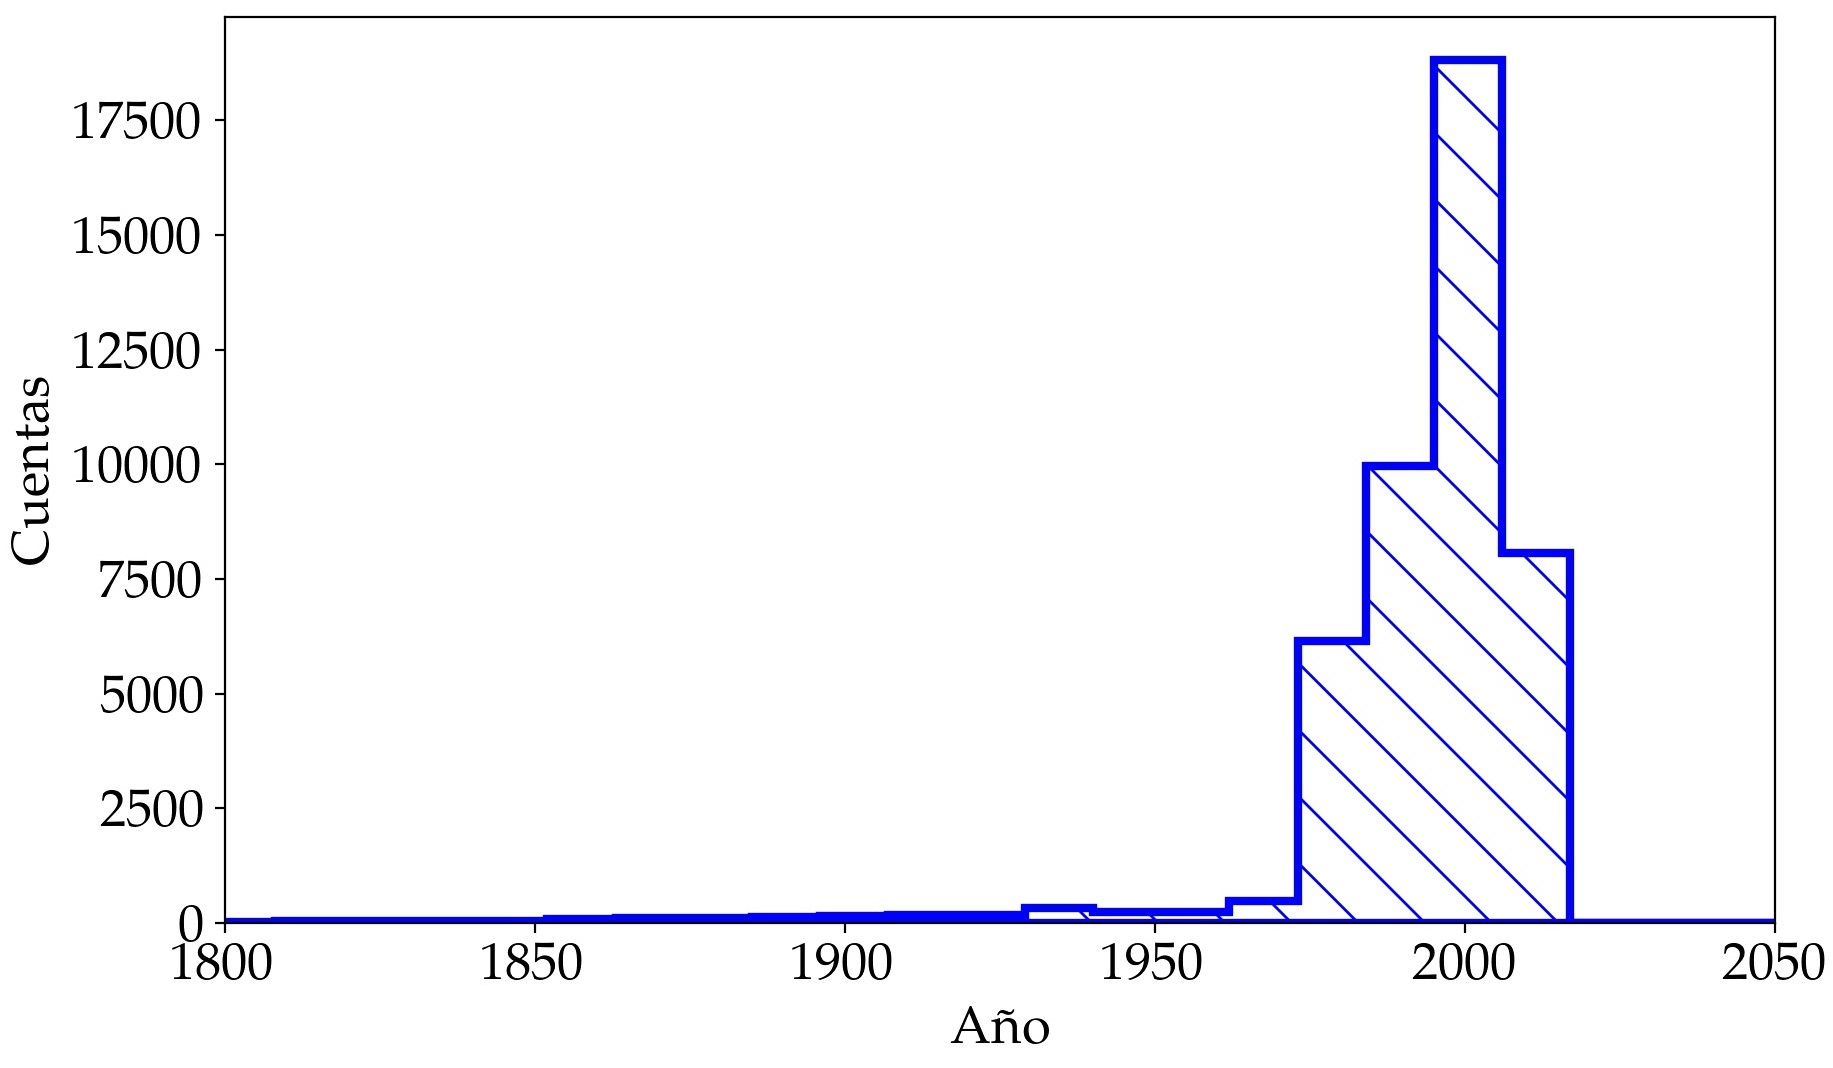
\includegraphics[scale = 0.55]{year_distribution}
		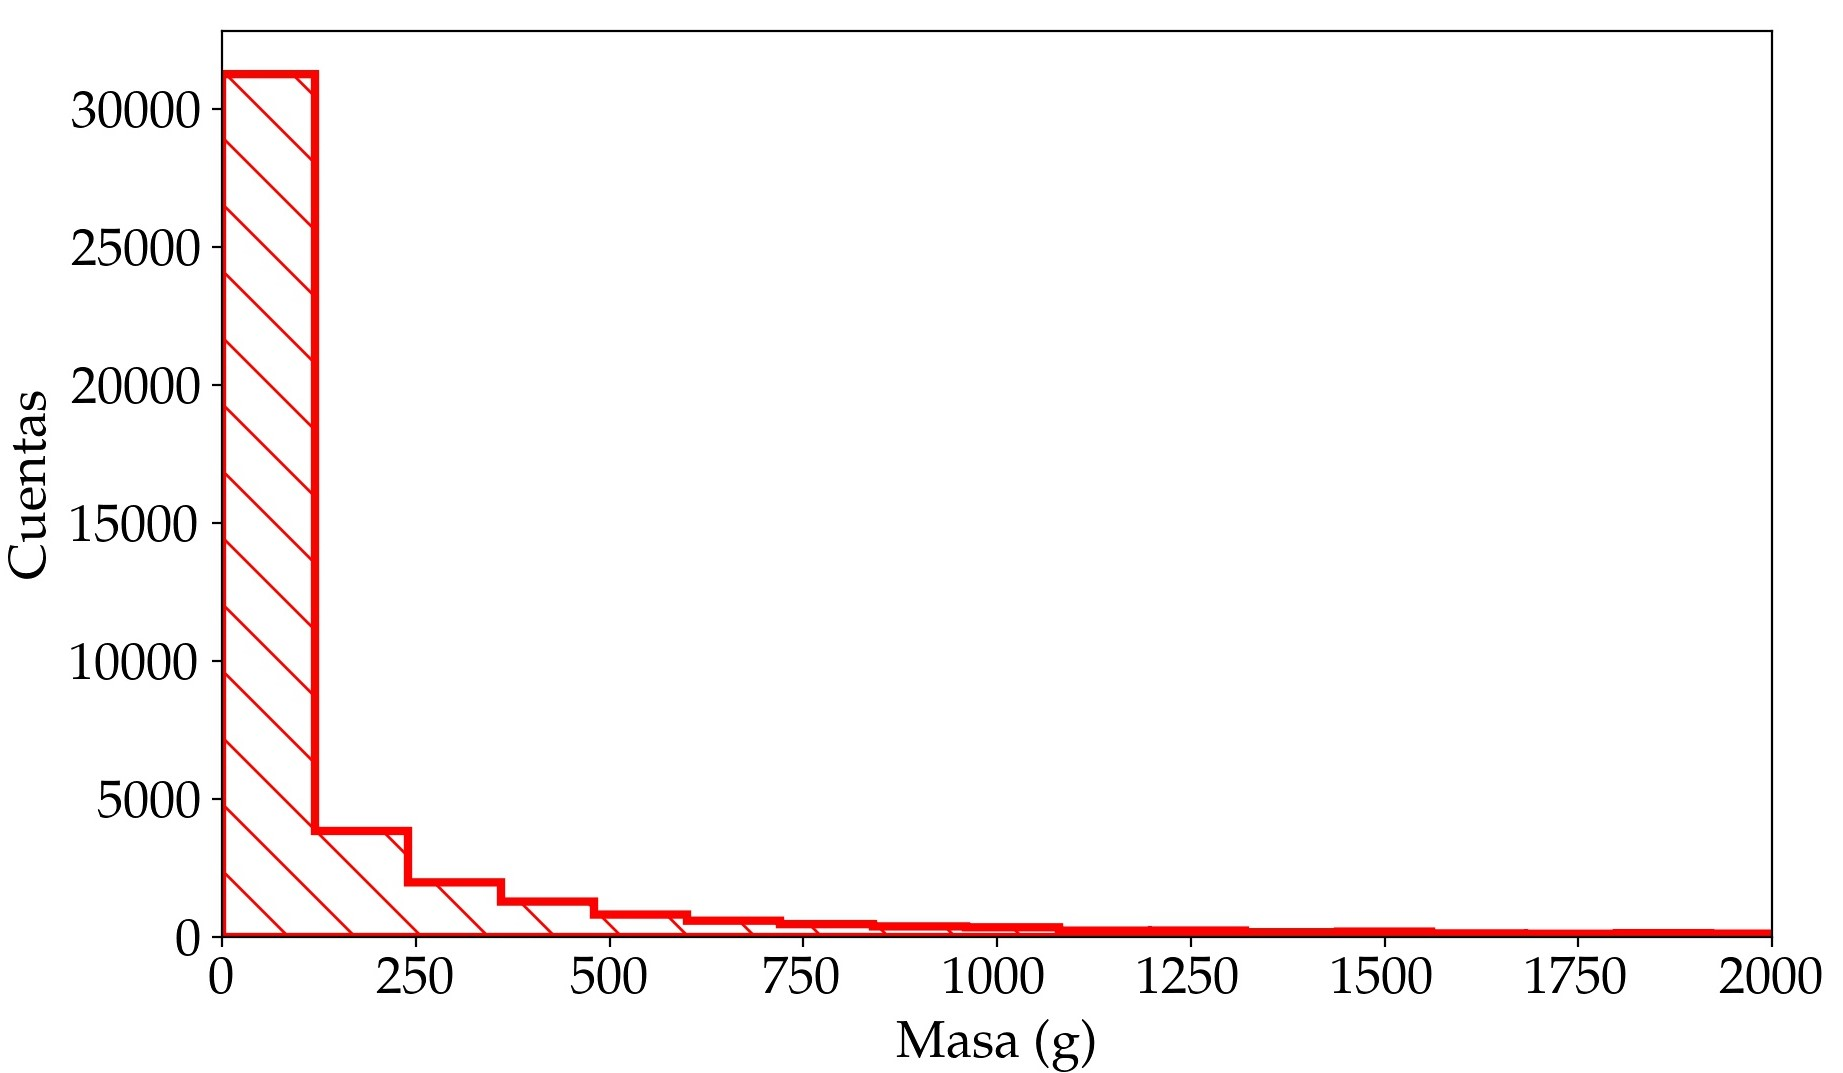
\includegraphics[scale = 0.55]{mass_distribution}
		\caption{(\textit{Arriba}): Representación gráfica de la variable año. (\textit{Debajo}): Representación gráfica de la variable masa.}
	\end{figure}
    En el caso de las variables categóricas, existe una que no admite una representación clara mediante diagrama de barras, que es la clasificación geológica del meteorito. Esto es debido a que se trata de una variable con 466 categorías, que resulta imposible administrar mediante un diagrama de barras.\\
    La otra variable categórica de interés es una variable binaria que indica si el meteorito fue descubierto en su caída o si por el contrario fue descubierto una vez había caído. Puede ser interesante relacionar esta variable con la localización o el año. En la \hyperref[Fig:year_fall]{Fig. 2} se representa el cambio en la distribución de la variable año en función de si el meteorito fue detectado en su caída o encontrado posteriormente. Aquí se observa un fenómeno interesante, la causa de que existan gran cantidad de meteoritos descubiertos en los últimos años no se debe a un aumento de la cantidad de meteoritos que caen del cielo, sino a que la mayoría de ellos son descubrimientos de meteoritos que cayeron anteriormente. Si nos fijamos en la distribución de los meteoritos descubiertos en su caída, ésta se mantiene constante.\\
    Falta por describir la variable central de este análisis, la localización geográfica de cada meteorito. En la \hyperref[Fig:geolocation]{Fig. 3} se puede ver la distribución de las variables latitud y longitud que definen la geolocalización sobre el mapa mundial. Se observa como, a pesar de lo que se podría esperar, la densidad de meteoritos por unidad de área no es homogénea. En teoría, un meteorito no elige caer en Estados Unidos o en Europa, ni evita a toda costa caer en el Amazonas. La conclusión que se extrae de esta distribución heterogénea, es que en aquellas zonas donde no se observan muchos meteoritos deben quedar muchos por descubrir.
    \begin{figure}[t]
    	\centering
    	\label{Fig:year_fall}
    	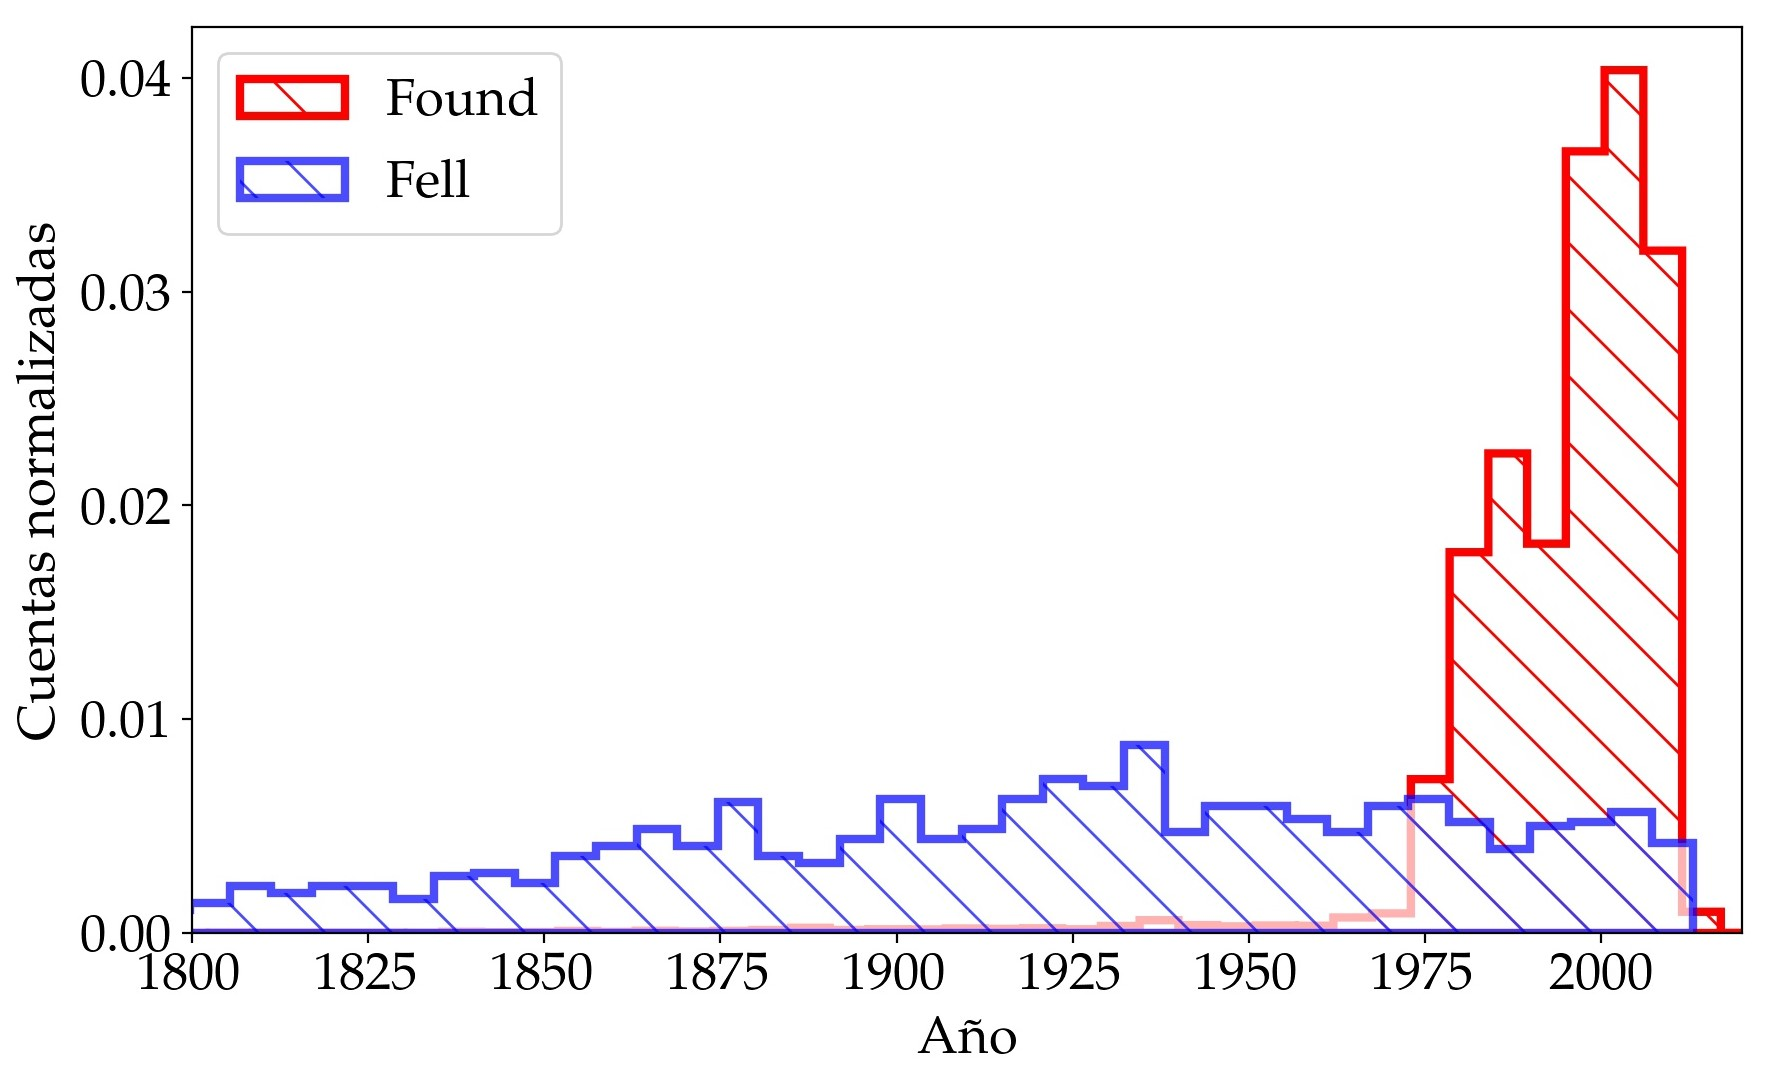
\includegraphics[scale = 0.55]{year_vs_fall}
    	\caption{Distribución de la variable año en función de la variable categórica binaria \textit{fall}.}
    \end{figure}
    Una gráfica que puede arrojar algo de luz a esta suposición es la representación de la variable de localización geográfica conjuntamente con la variable \textit{fall}. Dicha gráfica se muestra en la \hyperref[Fig:geo_fall]{Fig. 4}. Se observa como aquellas aglomeraciones con mayor densidad de meteoritos por unidad de área están formadas en su mayor medida por descubrimientos, no por caídas. Evidentemente, los meteoritos detectados en su caída tampoco se distribuyen de forma homogénea, ya que es más fácil que se reporte la caída de un meteorito en aquellas regiones con mayor población. 
	\clearpage
	\begin{landscape}
		\begin{figure}[t]
			\centering
			\label{Fig:geolocation}
			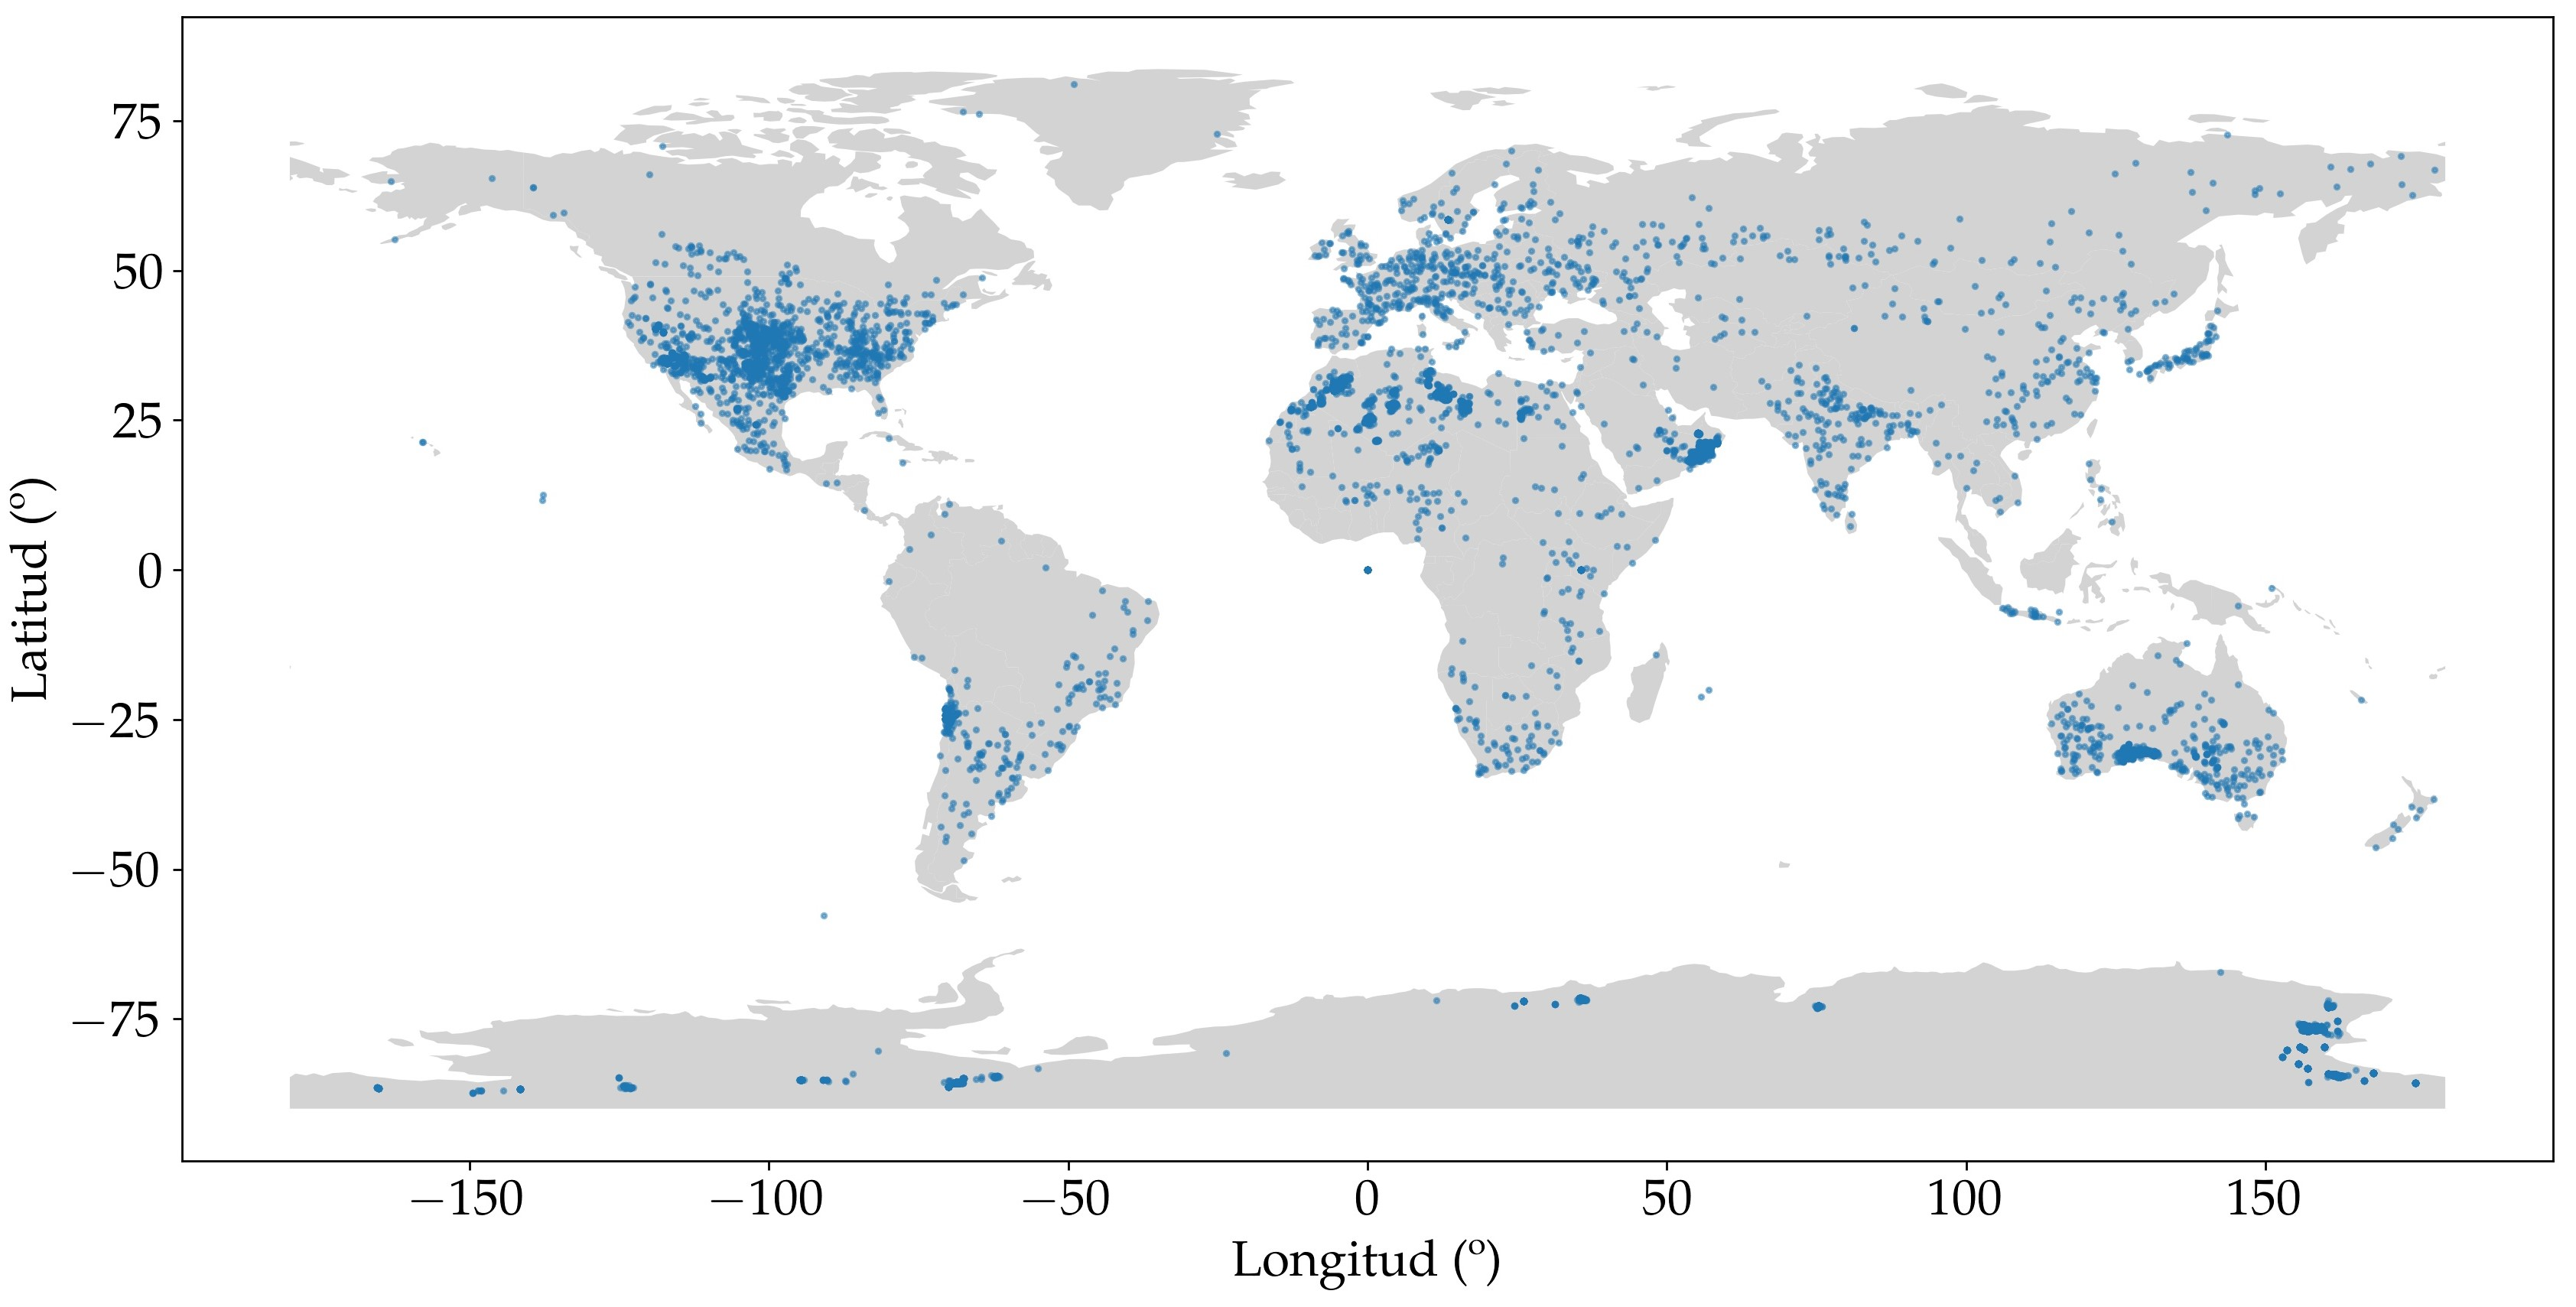
\includegraphics[scale=0.7]{geo_distribution}
			\caption{Localización geográfica de la caída de cada meteorito.}
		\end{figure}
	\clearpage
	    \begin{figure}[t]
	    	\centering
	    	\label{Fig:geo_fall}
	    	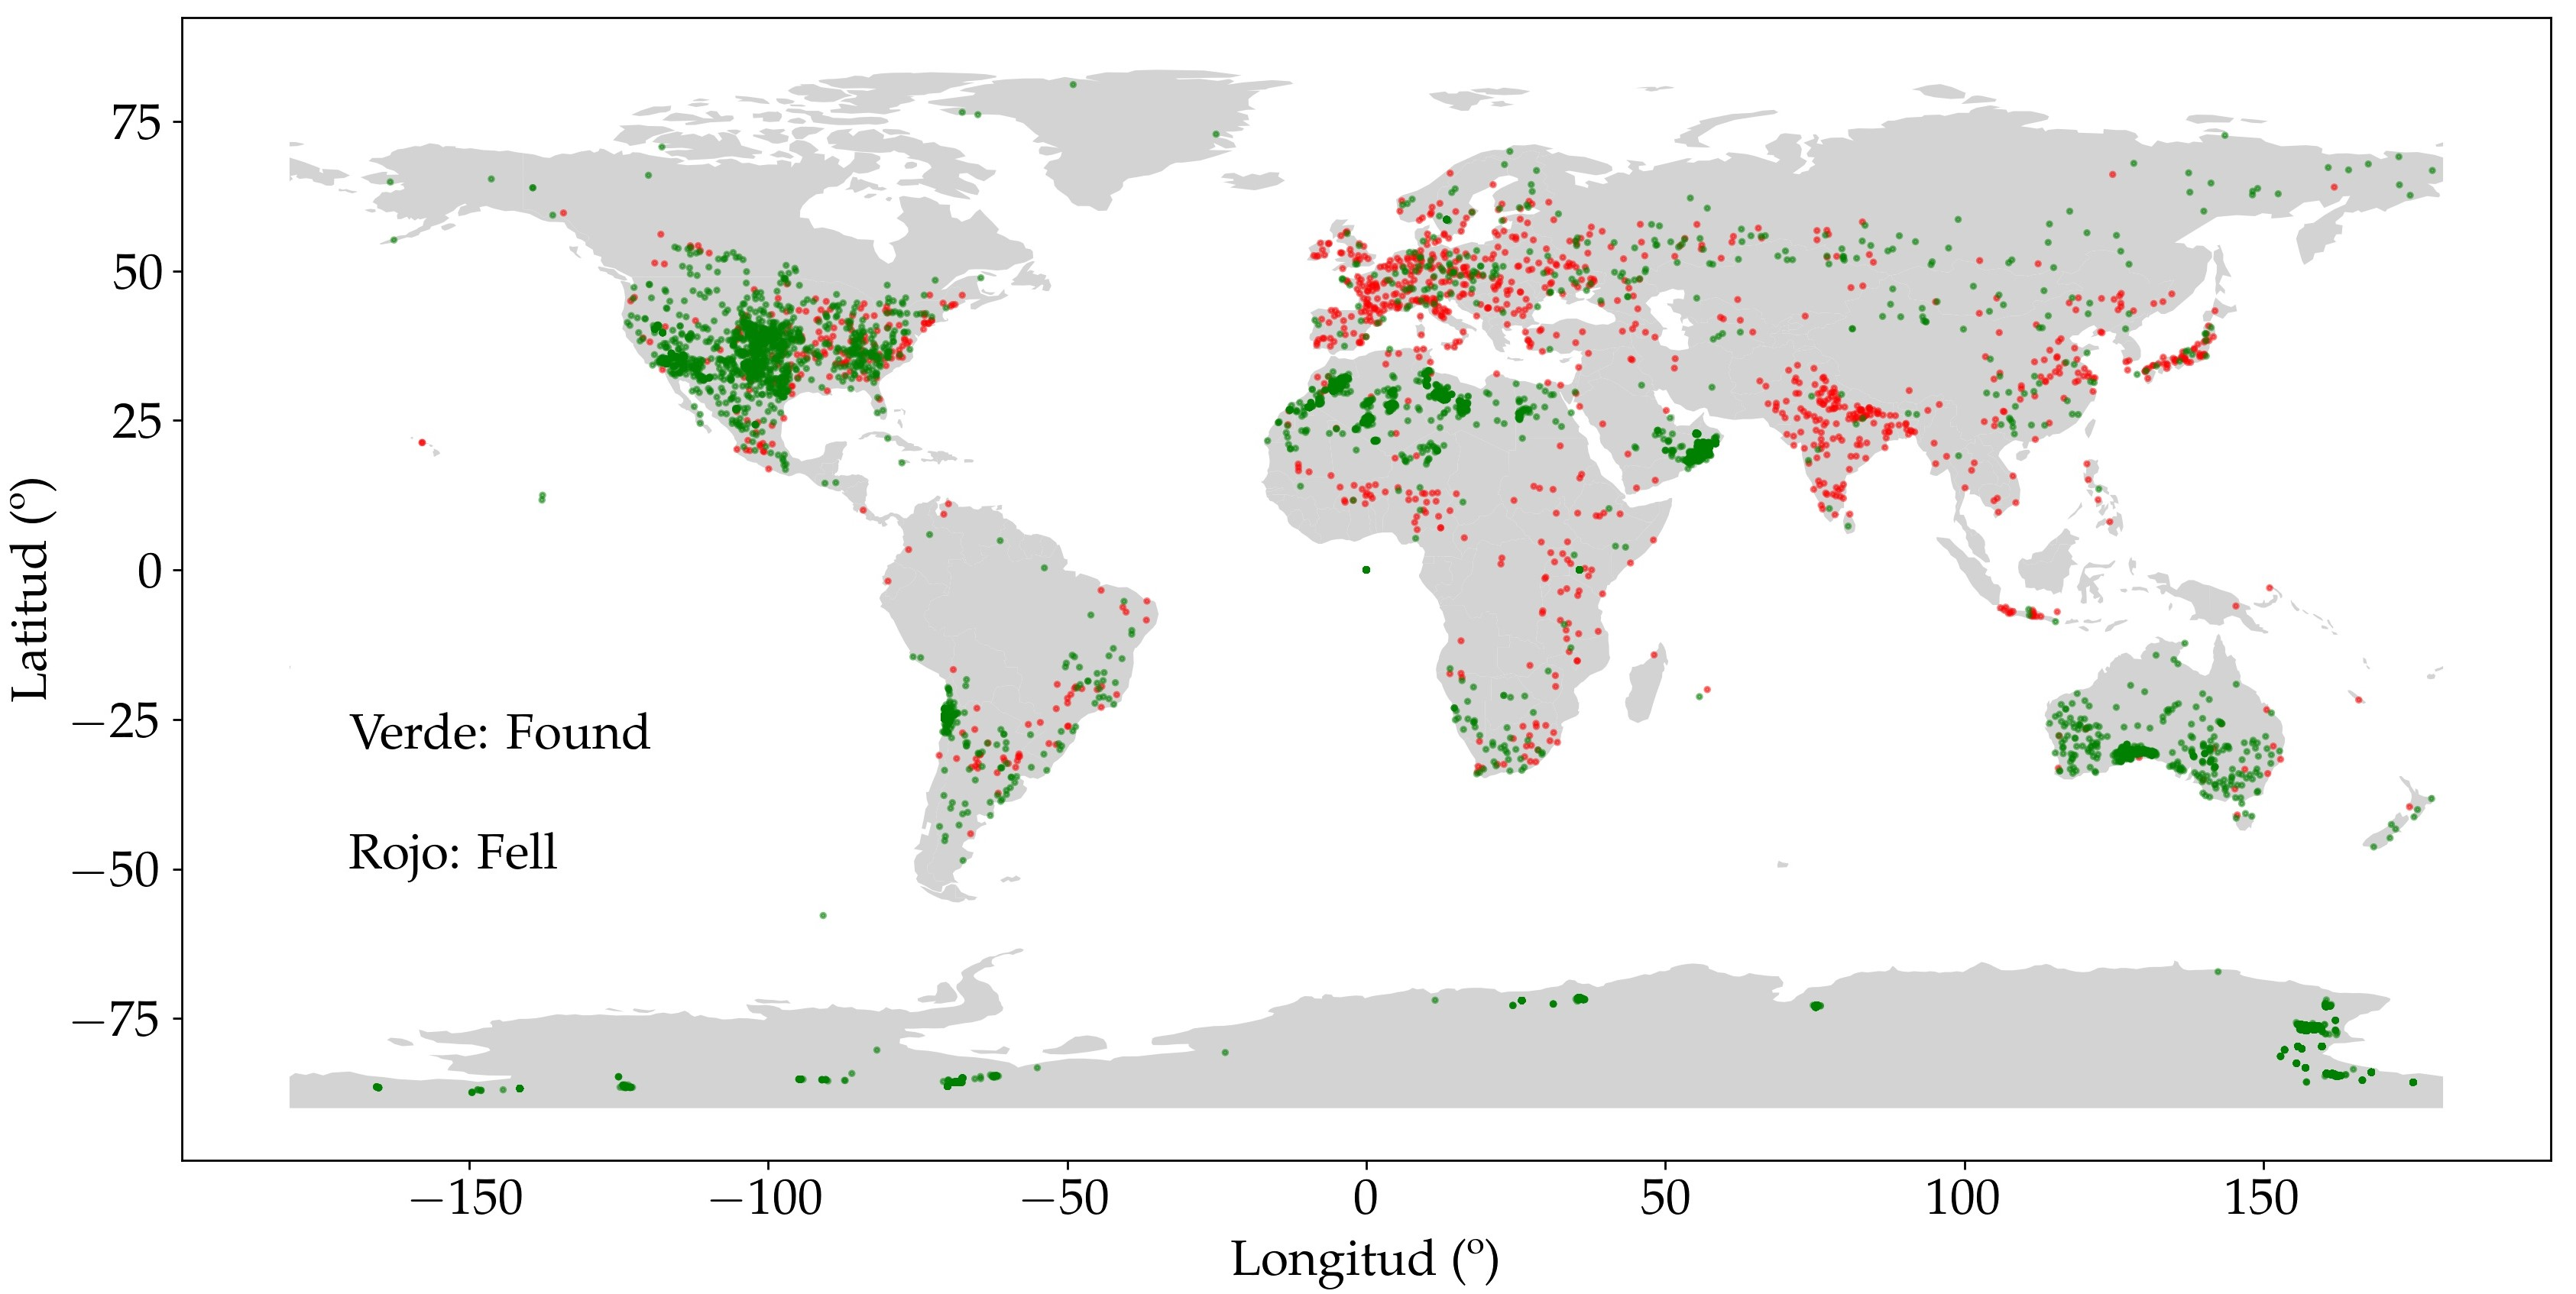
\includegraphics[scale=0.7]{geo_fall}
	    	\caption{Localización geográfica de la caída de cada meteorito en función de la variable \textit{fall}.}
	    \end{figure}
	\end{landscape}
    \section{Planteamiento de la visualización}
    Lo que se ha realizado hasta ahora es, a través de una exploración previa de los datos, establecer una serie de cuestiones y tratar de responderlas de forma gráfica. Sin embargo, las gráficas que se han aportado hasta ahora son estáticas y no permiten al usuario interactuar con ella.\\
    En esta sección se pretende realizar el planteamiento de una visualización de tipo \textit{dashboard} interactiva para representar los datos expuestos en el apartado anterior.\\
    Las preguntas que se pretende responder se pueden resumir en los siguientes puntos:
    \begin{itemize}
    	\item ¿Cómo se \textbf{distribuyen geográficamente} los meteoritos alrededor del mundo?
    	\item ¿\textbf{Cuándo} se descubrieron? 
    	\item ¿\textbf{Cómo} se descubrieron? Detectando su caída o encontrando sus restos.
    	\item ¿Cuánto \textbf{pesan}?
    \end{itemize}
	Una vez sabemos las preguntas que queremos responder y conocemos el conjunto de datos a través de su análisis exploratorio, podemos proceder a plantear qué visualizaciones queremos incluir en el \textit{dashboard} interactivo.
	\subsection{El mapa}
	La parte central del \textit{dashboard} la debe ocupar el \textbf{mapa mundi} con los datos de geolocalización sobre él, tal y como se muestra en las visualizaciones estáticas de la \hyperref[Fig:geolocation]{Fig. 3} y la \hyperref[Fig:geo_fall]{Fig. 4}. Para que la visualización represente la máxima información posible, se representará la variable \textbf{\textit{Fall}} mediante el color. Al ser una variable binaria, el usuario podrá observar fácilmente cómo se distribuyen ambas categorías en el mapa. Esta propuesta sería factible para cualquier variable categórica, como por ejemplo la \textbf{clasificación geológica}, sin embargo, debido a que la clasificación geológica posee 466 categorías, resultaría imposible que cualquier usuario de la visualización pudiera extraer respuestas del color de los puntos en el mapa. Por tanto, la variable que hace referencia a la clasificación geológica se encuentra disponible como etiqueta desplegable, es decir, si el usuario decide picar con el ratón sobre cualquier punto (meteorito) del mapa, se desplegará una etiqueta que contendrá la clasificación geológica de dicho meteorito. En cuanto a las variables numéricas continuas (\textbf{masa y año}), se podrían representar utilizando el tamaño del punto, que tendría sentido sobretodo en el caso de la masa. Sin embargo, al tener una distribución de masas tan desbalanceada, donde la mayoría de los meteoritos poseen una masa muy pequeña en comparación con los meteoritos más pesados, que son extremadamente escasos, se ha decidido no emplear esta técnica. Ambos, año y masa, se colocan, junto al nombre del meteorito y su clasificación geológica, en la ya mencionada etiqueta desplegable.\\
	Esta parte de la visualización pretende responder la primera de las preguntas planteada: ¿Cómo se distribuyen los meteoritos alrededor del mundo?
	\subsection{Diagrama de dispersión año VS masa}
	Un diagrama de dispersión sirve para observar en una misma gráfica tres aspectos a partir de dos variables continuas:
	\begin{itemize}
		\item La \textbf{distribución} de los datos a lo largo \textbf{de la primera variable}. En este caso la distribución de los meteoritos en el tiempo (año).
		\item La \textbf{distribución} de los datos \textbf{en la segunda variable}. En este caso la distribución de la masa de los meteoritos.
		\item La \textbf{relación entre ambas variables}, la masa en función del año.
	\end{itemize}	
	Aunque el tercero de estos puntos no responde a ninguna de las preguntas que se han planteado, no está de más añadir este tipo de respuestas a nuestro \textit{dashboard}. No se ha planteado como pregunta porque no se espera visualizar correlación entre las variables año y masa. Sí se han planteado las dos primeras: distribución de la masa y el año de forma independiente. Cabe destacar que la distribución de la variable año se complementará con un histograma.\\
	A la hora de elaborar un diagrama de dispersión (y cualquier gráfica que involucre variables numéricas), es importante reflexionar sobre la \textbf{escala} en la que es más adecuado representar cada variable. La variable año, aunque es cierto que la mayoría de los meteoritos se han descubierto a partir de 1950, no conviene transformarla. En el caso de la variable masa, sí que admite una transformación evidente. Si observamos su distribución (\hyperref[Fig:year_mass]{Fig. 1}) queda de manifiesto que la representación gráfica de esta variable se beneficiaría enormemente de una \textbf{transformación logarítmica}. De lo contrario las observaciones estarían mayoritariamente acumuladas en el eje $ Mass = 0 $, impidiendo al usuario observar correctamente los detalles de la distribución de los datos.\\
	Una vez establecidos los ejes, podemos plantearnos introducir más variables en la visualización a través del color, la forma o el tamaño del punto. Se ha decidido, en aras de conservar el mismo estilo seguido en el diseño del mapa, incluir la \textbf{variable \textit{Fall} a través del color}. Empleando además los mismos colores. De esta forma, al realizar consultas o filtrado de los datos, al usuario le resultará más sencillo extraer conclusiones globales sin necesidad de tener que acudir a la leyenda de cada gráfica del \textit{dashboard}.
	\subsection{Histograma en la variable año}
	Aunque se haya representado la distribución de ambas variables en la visualización anterior, para complementar la respuesta a la segunda pregunta (¿Cuándo se han descubierto los meteoritos?) se representa un histograma de la \textbf{variable año}. Esto se realiza de esta forma, ya que en el diagrama de dispersión, si no se realiza un filtrado de los datos muy exhaustivo sobre los datos que corresponden a años actuales, los puntos se aglomeran demasiado como para que el usuario pueda deducir la distribución de la variable año apoyándose únicamente en ese diagrama. 
	\subsection{Barras de filtrado}
	Además de estas tres visualizaciones, que son las principales del \textit{dashboard}, sobre todo la del mapa mundi, se proponen dos visualizaciones auxiliares que servirán en mayor medida para controlar el filtrado de los datos de forma cómoda para el usuario sobre las variables año y \textit{fall}. Cabe comentar que el filtrado en base a la localización geográfica se realiza sobre el propio mapa.\\
	La primera de estas dos visualizaciones es un \textbf{diagrama de barras sobre la variable categórica \textit{fall}}, que al ser binaria produce un diagrama con dos columnas que es fácilmente acoplable a uno de los lados del \textit{dashboard}. Pretende responder la tercera pregunta planteada, ¿Cómo se descubrieron los meteoritos? Dicho diagrama de barras se representa en \textbf{escala logarítmica} debido a la diferencia tan grande entre el número de meteoritos en cada clase. Además, por cuestiones de armonía para con el resto de visualizaciones del \textit{dashboard}, cada barra se representa con el color que se asignó en el resto de gráficas a las dos clases. Si el usuario desea filtrar los datos para representar únicamente los meteoritos que fueron detectados en su caída y excluir los descubiertos con posterioridad, solo tiene que pulsar sobre la barra de la clase \textit{Fell}.\\
	La otra gráfica es una línea que contiene únicamente las observaciones de la \textbf{variable año representadas en una dimensión}. El único objetivo de esta visualización es que el usuario pueda \textbf{filtrar fácilmente} los datos en la variable tiempo definiendo un intervalo con el ratón. 
	\subsection{Distribución espacial}
	La distribución espacial de cada uno de los elementos anteriormente descritos en el \textit{dashboard} puede consultarse en la \hyperref[Fig:borrador]{Fig. 5}.
	\clearpage
	\begin{landscape}
		\begin{figure}[t]
			\centering
			\label{Fig:borrador}
			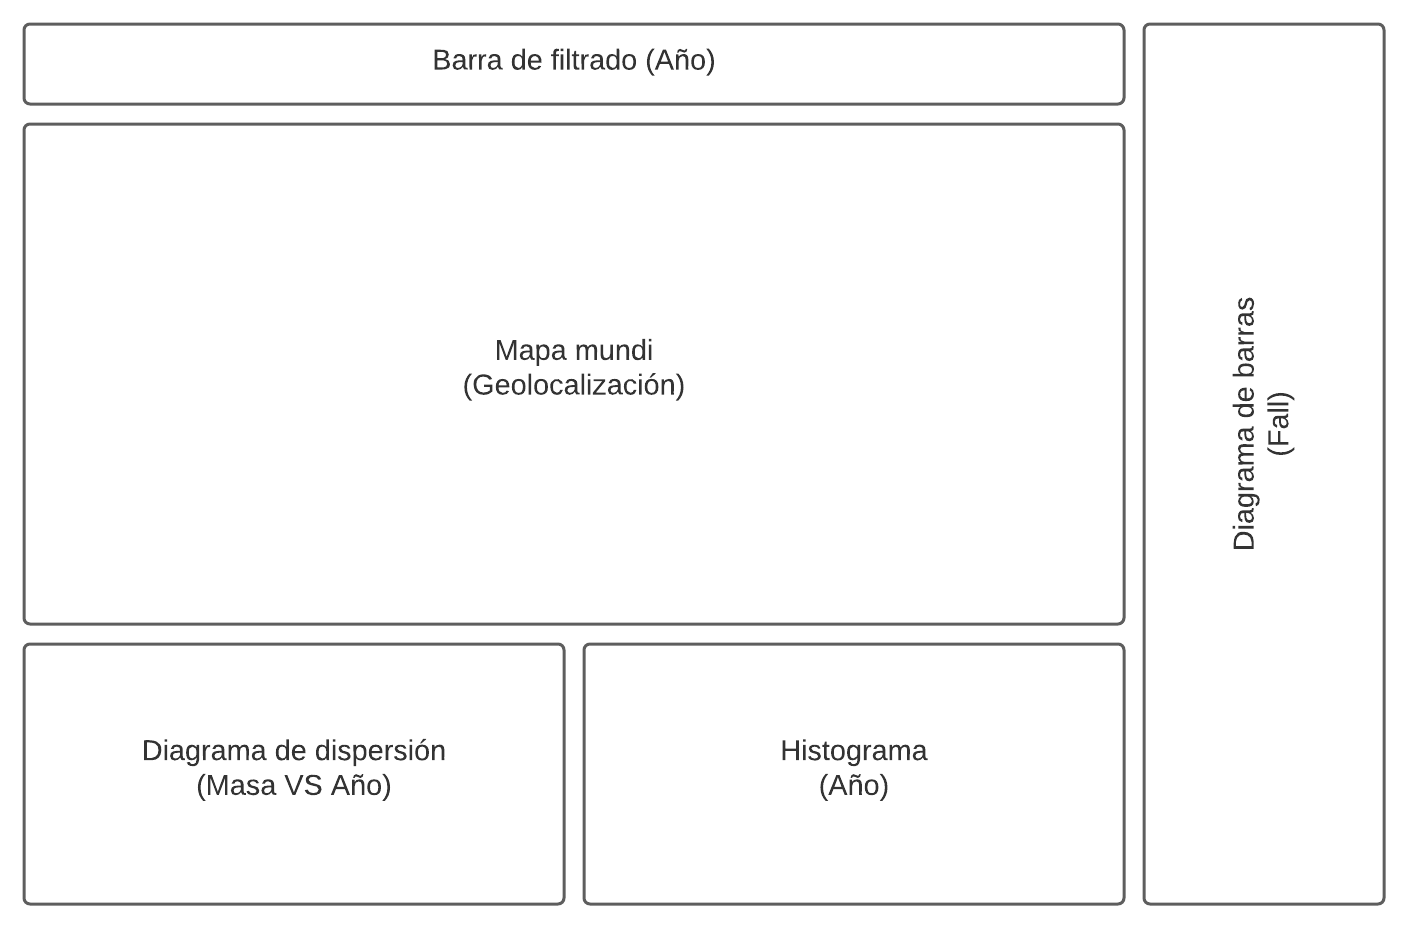
\includegraphics[scale=1]{borrador}
			\caption{Distribución espacial de cada visualización dentro del \textit{dashboard}.}
		\end{figure}
	\end{landscape}
	\clearpage
	\section{Implementación}
	La implementación del \textit{dashboard} se ha realizado utilizando el \textit{software} especializado en visualizaciones Tableau. La carga de los datos se realiza importando el archivo como datos geoespaciales. Cabe reseñar que para poder realizar el \textit{dashboard} con todas las prestaciones disponibles, se ha decidido cambiar los datos de formato CSV a GeoJSON. De este modo la herramienta Tableau es capaz de reconocerlos de forma automática como datos geoespaciales. La estructura del archivo GeoJSON seleccionada ha sido la siguiente: 
	\begin{lstlisting}
		{
			"type": "FeatureCollection",
			"features": [
			{
				"type": "Feature",
				"geometry": {
					"type": "Point",
					"coordinates":  [ 6.083330,50.775000 ]
				},
				"properties": {
					"name":"Aachen",
					"id":1,
					"nametype":"Valid",
					"recclass":"L5",
					"mass":"21",
					"fall":"Fell",
					"year":1880,
					"GeoLocation":"(50.775000, 6.083330)"
				}
			},
	\end{lstlisting}
    Una vez se tienen los datos en este nuevo formato, se importa el archivo directamente en Tableau, que reconoce automáticamente el carácter geoespacial de los mismos, y se comienzan a diseñar cada una de las visualizaciones descritas en la sección anterior.\\
    A continuación se describen todas ellas individualmente. Cada una ha sido implementada en una hoja de Tableau. El \textit{dashboard} final es el resultado de realizar una composición con todas ellas.
    \subsection{El mapa}
    La representación geográfica de los datos en el mapa se realiza gracias a las prestaciones que aporta Tableau para trabajar con datos geoespaciales. El mapa de fondo es colocado automáticamente por Tableau al seleccionar representar la variable Geometry de tipo geoespacial. Esta ventaja es la que justifica el cambio de formato de los datos de CSV a GeoJSON.\\
    \begin{figure}[h]
    	\centering
    	\label{Fig:mapa}
    	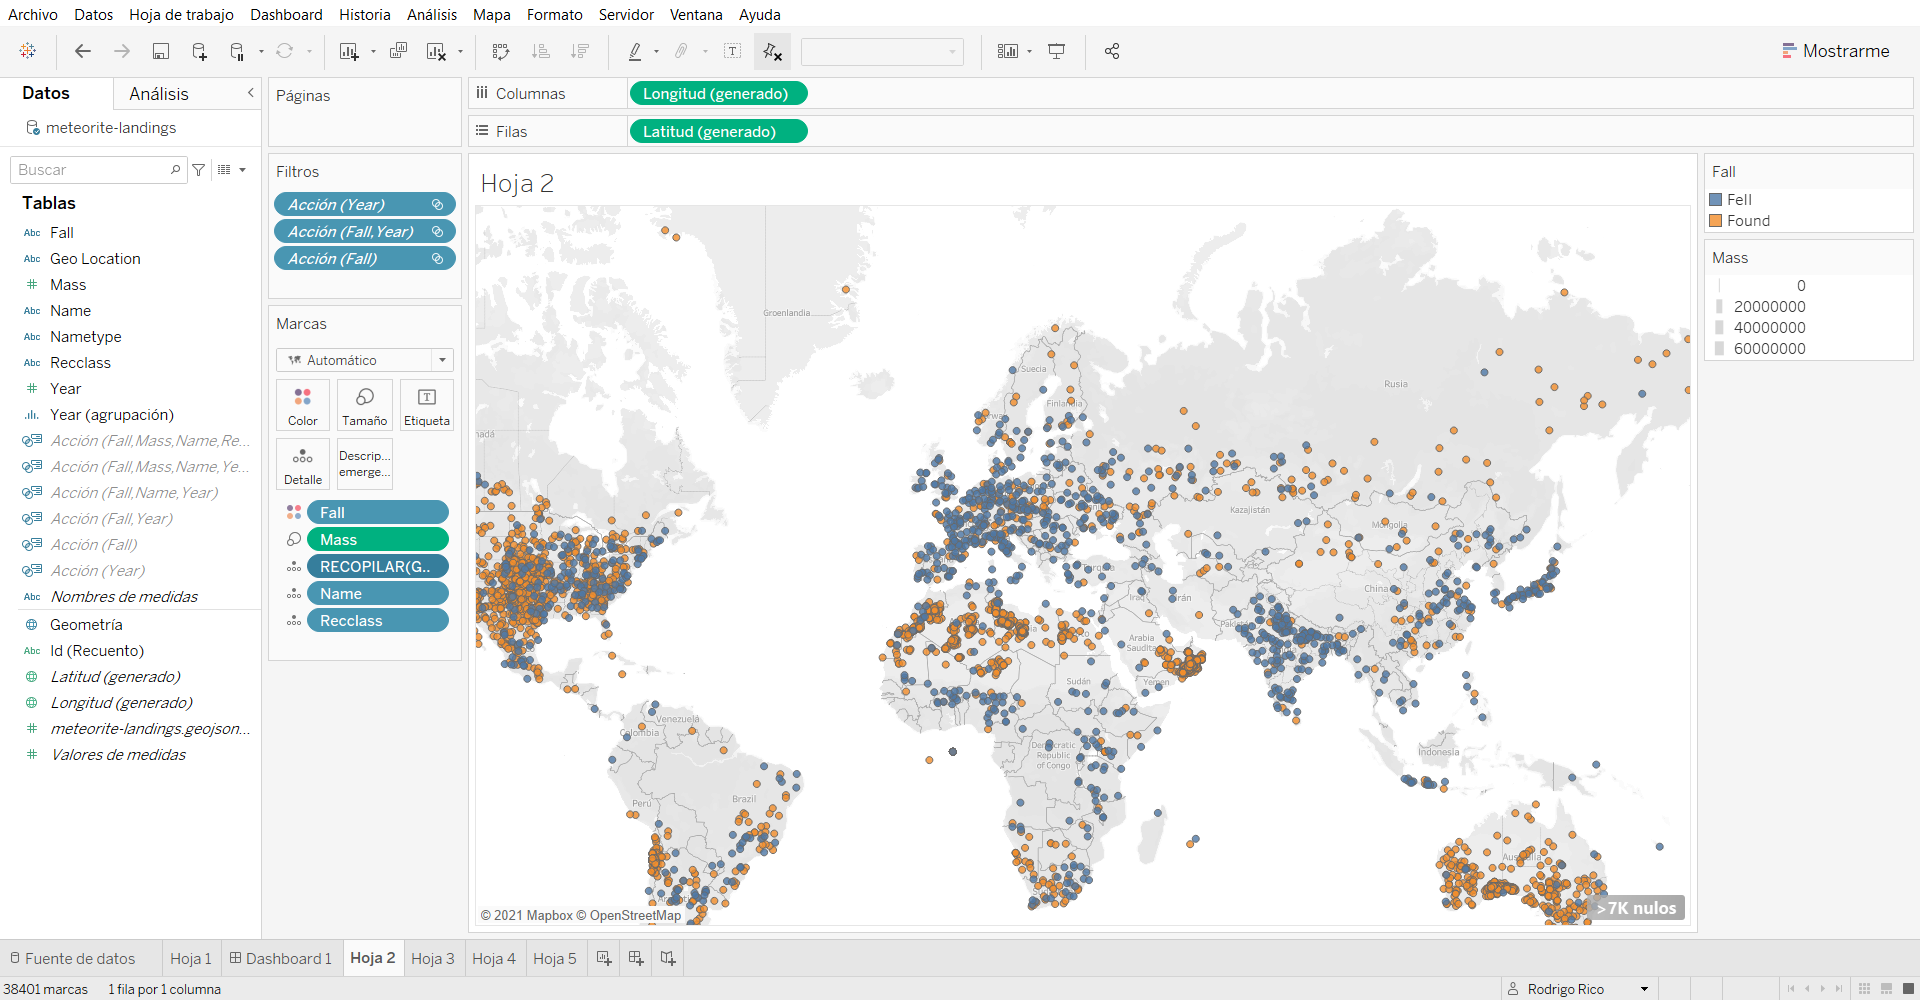
\includegraphics[width=\textwidth]{Captura de pantalla (63)}
    	\caption{Creación de la visualización del mapa desde en entorno de Tableau.}
    \end{figure}
    \\
	Esta visualización permite al usuario interactuar con los datos localizados alrededor del mapa mundi. El usuario puede encuadrar una región concreta del mapa o seleccionar un meteorito concreto de manera que se desplieguen sus datos.
	\subsection{Diagrama de dispersión}
	El diagrama de dispersión se realiza seleccionando la variable año como columna y la variable masa como fila. Posteriormente se selecciona la opción de realizar un diagrama de dispersión y modifica en este caso la escala del eje Y a logarítmica.\\
	\begin{figure}[h]
		\centering
		\label{Fig:dispersion}
		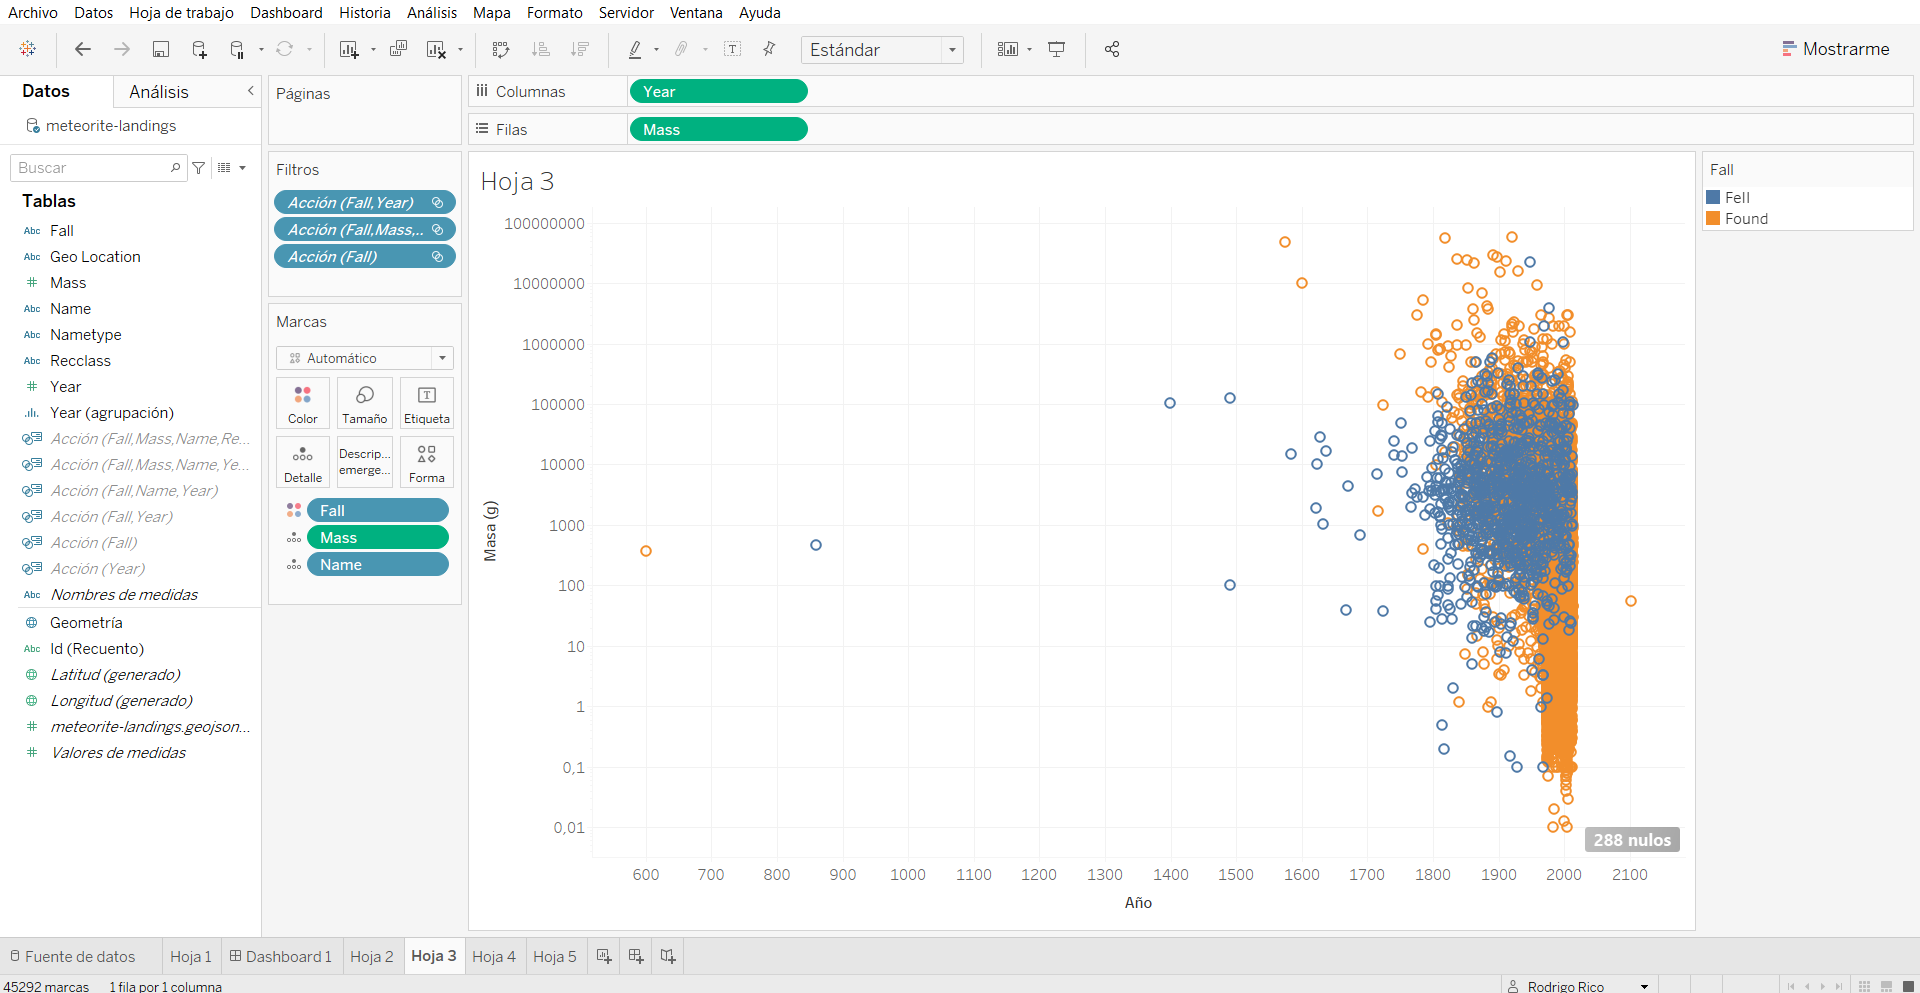
\includegraphics[width=\textwidth]{Captura de pantalla (64)}
		\caption{Creación de la visualización del diagrama de dispersión desde en entorno de Tableau.}
	\end{figure}
    \\
	Al igual que la visualización anterior, ésta permite que el usuario seleccione datos con el ratón para consultar sus propiedades de forma individual.
	\subsection{Histograma}
	Para la creación del histograma tenemos que crear dos variables derivadas. La primera para agrupar la variable año en celdas de 5 años y así definir el histograma sobre ese tamaño de celda. La segunda para definir la variable recuento. Ambas definiciones se realizan fácilmente utilizando las opciones que permite Tableau.\\
	\begin{figure}[h]
		\centering
		\label{Fig:histograma}
		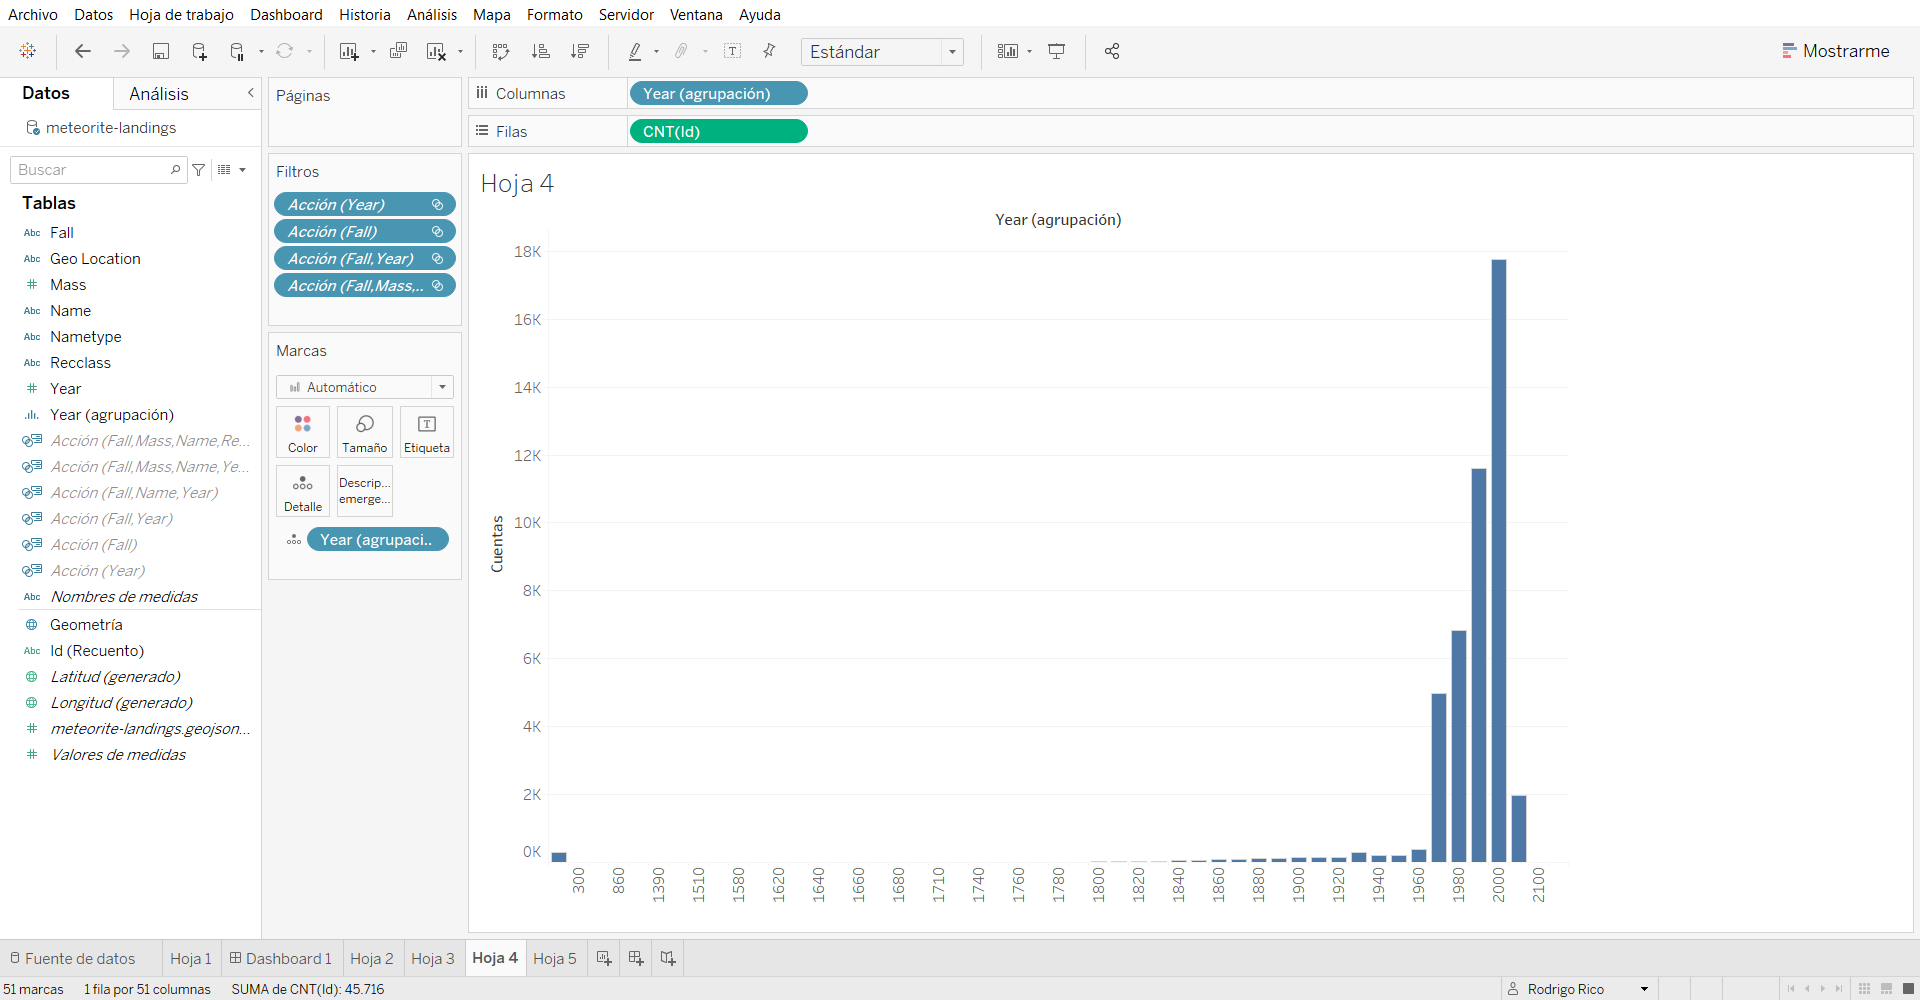
\includegraphics[width=\textwidth]{Captura de pantalla (65)}
		\caption{Creación de la visualización del histograma desde en entorno de Tableau.}
	\end{figure}
	\subsection{Diagrama de barras}
	El diagrama de barras se realiza introduciendo como columna la variable \textit{Fall} y como fila la variable recuento definida en la anterior visualización. Se selecciona la opción de Tableau para reproducir un diagrama de barras. Posteriormente se establece la escala logarítmica para la variable recuento.\\
	\begin{figure}[h]
		\centering
		\label{Fig:barras}
		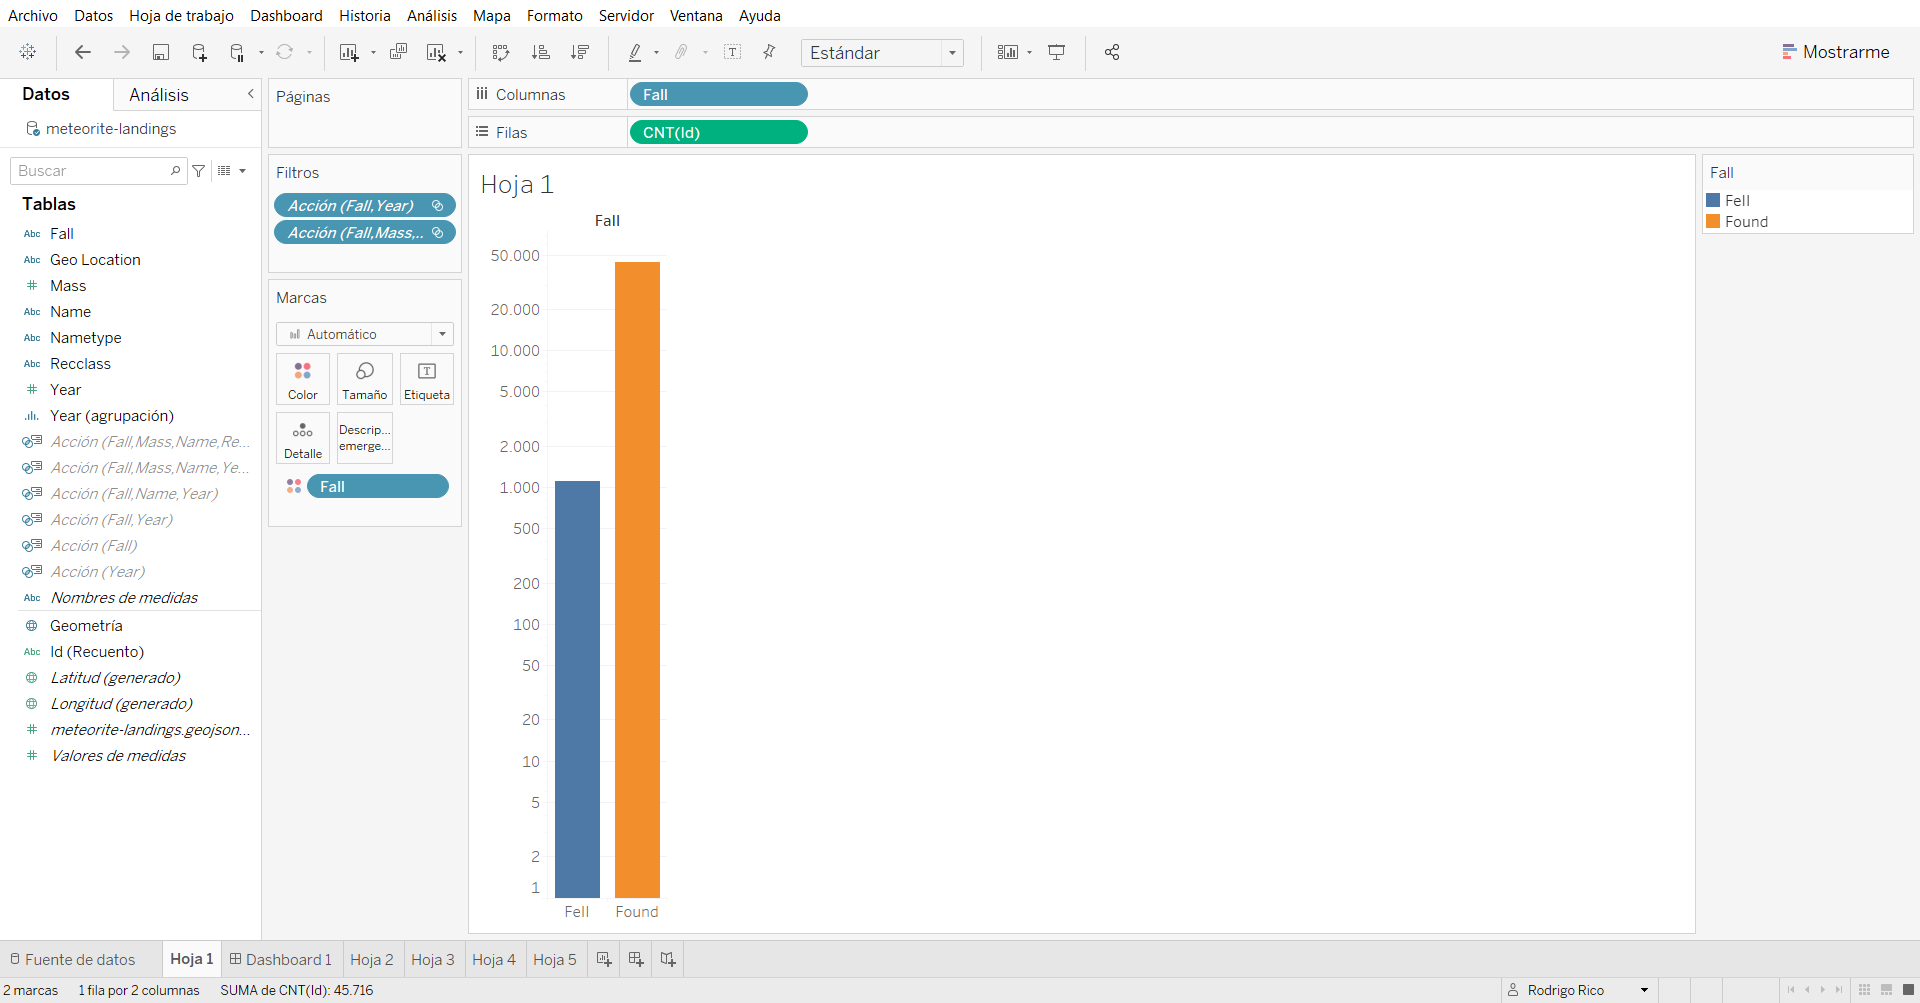
\includegraphics[width=\textwidth]{Captura de pantalla (66)}
		\caption{Creación de la visualización del diagrama de barras desde en entorno de Tableau.}
	\end{figure}
	\\
	Esta visualización permite filtrar los datos de todo el \textit{dashboard} en función del valor de la variable \textit{Fall} seleccionando una de las dos barras del diagrama.
	\clearpage
	\section{Dashboard}
	Una vez implementadas todas las visualizaciones que componen el \textit{dashboard}, siguiendo el borrador de la \hyperref[Fig:borrador]{Fig. 5}, se colocan todas ellas para formar la composición final:\\
	\begin{figure}[h]
		\centering
		\label{Fig:dashboard}
		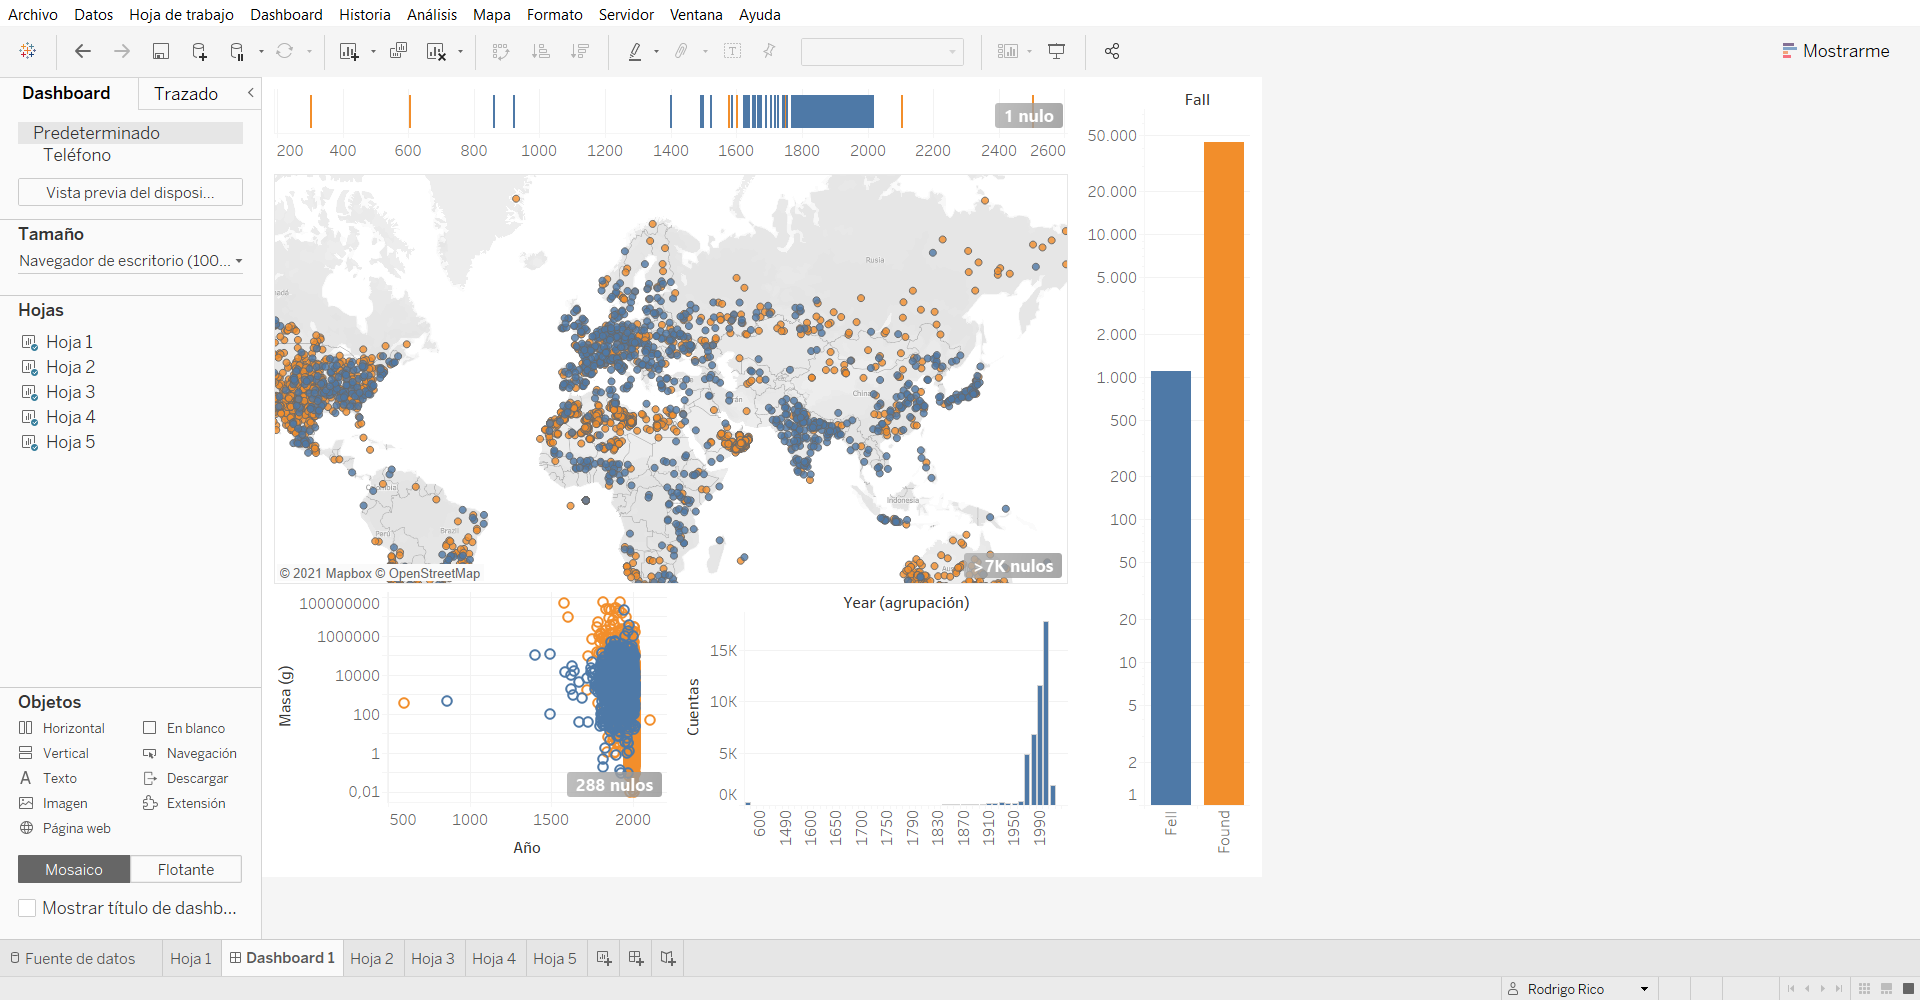
\includegraphics[width=\textwidth]{Captura de pantalla (67)}
		\caption{Creación de la visualización del \textit{dashboard} desde en entorno de Tableau.}
	\end{figure}
	\\
	\href{https://dub01.online.tableau.com/#/site/rodrigoricogomez/workbooks/612901?:origin=card_share_link}{Enlace al dashboard}\\
	
	
	
	
	
	
	
	
\end{document}